\documentclass[sigplan,nonacm]{acmart}
% Use option lineno for line numbers 

\title{Efficient Maritime Object Detection: YOLOv7 Tuning and Ghost Convolution Integration}

\author{James Bebarski}
\affiliation{%
    \institution{Roux Institute at Northeastern University}
    \city{Portland}
    \state{Maine}
    \country{USA}
}
\email{bebarski.j@northeastern.edu}

\author{David Getchell}
\affiliation{%
    \institution{Roux Institute at Northeastern University}
    \city{Portland}
    \state{Maine}
    \country{USA}
\email{getchell.da@northeastern.edu}
}
\keywords{computer vision, object detection, supervised machine learning, YOLOv7, Ghost Convolutions, Real-Time Systems}

\begin{document}



\begin{abstract}
\textit{Object detection plays a crucial role in various industries, including maritime safety. This paper details the development and optimization of an object detection system specifically designed for naval environments in collaboration with Lookout, a Massachusetts-based company. Initially, we fine-tuned hyper-parameters on the standard YOLOv7 architecture, achieving significant improvements in precision and recall. Building on this success, we explored developing a more lightweight model by integrating Ghost convolution modules, which drastically reduced computational demands while maintaining a relatively high degree of precision and recall. Our enhanced model, tested on maritime-specific datasets, demonstrated strong performance, particularly in detecting boats and jet skis, making it suitable for deployment in resource-constrained, real-world applications. This work offers a cost-effective solution for advancing boating safety through innovative object detection technology.}
\end{abstract}




\maketitle

\section*{Introduction}
Object detection is a major area of research in the rapidly evolving field of computer vision with a broad set of applications, from autonomous vehicles to augmented reality. In this project, we explored how object detection can be applied to decrease maritime safety incidents. Our class had the opportunity to partner with Lookout, a company seeking to leverage object detection to improve boater safety out on the water.  

Lookout's main product is a head-up display that, among other things, provides boaters with real-time alerts about potential hazards or objects on the water, such as boats, jet skis, swimmers, buoys, and lifesaving appliances. By partnering with Lookout, our project was not just a a technical challenge to see who could get the best results, but a business-driven problem. Our goal was not only to achieve high results in critical metrics but also to explore methods to make such a system viable for deployment in more resource-constrained environments. By aiming to reduce computational load, we believed this would positively impact the feasibility and cost-effectiveness of their product or a product like theirs. 

Our approach began with fine-tuning the hyper-parameters of the standard YOLOv7 architecture to work with the data set that Lookout provided. Adjustments to the hyper-parameters alone led to noticeable improvements in precision, recall, and mAP50 over the baseline YOLOv7 run. However, the practical challenges of deploying such a model in real-world settings, such as computational load, led us to exploring optimizations beyond the standard YOLOv7 architecture. Our goal was to reduce computation demands while providing a comparable level of performance. 

This focus led us to Ghost convolution modules, which were designed to generate feature representations/maps similar to standard convolutions but with significantly fewer parameters and floating point operations per second (FLOPS). We recognized the potential of these modules to help us develop our lighter model, which we have dubbed "Big Ghost," where all the standard convolution modules have been replaced with Ghost modules. 

By bringing the hyper-parameter adjustments from our initial YOLOv7 work into the development of Big Ghost, we aimed to achieve a model that not only performed well but also aligned with the business needs of deploying a cost-effective and efficient solution in real-world maritime safety applications. 

\section*{Background}
Object detection on the water presents unique challenges compared to other domains like urban settings or indoor scenes. The sea's ever-changing nature, varying weather conditions, and the presence of many other diverse objects, like boats, jet skis, buoys, and swimmers, make accurate detection a pretty complex task. Additionally challenging for object detection in marine settings is the presence of a limited range of pixel values, with the ocean, the horizon, and the sky being various shades of blue. Traditional object detection models often need help with the variability and unpredictability of maritime scenes, necessitating a tailored solution. 

The YOLOv7 object detection framework is touted for its balance, speed, and accuracy, and it has been widely used in various applications similar to ours. However, its standard architecture, albeit powerful, can be demanding computationally, particularly in resource-constrained environments like those encountered in maritime safety systems. In the business world, we should strive to get more with less, and if we can reach a comparable level of performance with fewer resources, we should pursue that route. 

Another challenge to consider is balancing processing power and energy efficiency. While larger vessels and their owners may feel comfortable making an investment to meet the needs of YOLOv7 or models like it, other smaller vessels - such as jet skis - could also benefit from this sort of technology but lack the same ability to accommodate the demands of more computationally intensive products. The potential impact of this development would be significant if some of Lookout's features could be optimized to run on hardware similar to that of a high-end smartphone. Having the ability to integrate these kinds of advanced safety features on smaller vessels with a smaller physical footprint would be an ideal outcome. 

\section*{Methods and Analysis}
We found that integrating ghost modules into a convolutional neural network similar to YOLOv7 can help mitigate some of the challenges associated with traditional convolution layers. These modules generate comparable feature maps to standard convolution layers but with significantly fewer parameters and floating point operations per second (FLOPS), making them particularly useful for the purposes and vision of our project. The beauty of ghost modules is that they could easily replace a standard convolutional module, as they require the identical input tensors as their relatives, and do not require tweaks to the tensor input and outputs that would be necessary if we decided to rebuild the architecture from the ground up completely. It was as simple as swapping out one for another. In fact, ghost modules were specifically designed to be a "plug and play" component in existing convolutional neural networks \cite{han2020ghostnet} .

We wanted to demonstrate how simple it was to change this architecture. In Figure 1, we provide two simplified diagrams showing the structural similarity between the YOLOv7 and Big Ghost architectures. These diagrams illustrate how straightforward it was to replace standard convolutional layers with Ghost modules. 

As you can see in Figure 1, the standard YOLOv7 architecture consists of 407 layers, 37,221,635 parameters, and 105.2 GFLOPS, while the Big Ghost architecture has 810 layers, 26,130,118 parameters, and 64.4 GFLOPS. The changes in our architecture compared to YOLOv7 resulted in nearly double the layers (99.02 percent more, to be precise), a 29.8 percent reduction in parameters, and a substantial 38.8 percent reduction in GFLOPS. The increase in layers, driven by the use of Ghost modules, helps our model to extract more detailed features without the same computational needs that are typically associated with these networks. This design aligns with our goal of providing a model with the ability to perform complex object detection tasks while simultaneously remaining efficient enough for deployment on resource-constrained maritime vessels like jet skis, kayaks, or smaller, less expensive boats. 

The inclusion of the additional layers presented a challenge in itself, as it can increase the risk of overfitting, a problem that we encountered and only accounted for later in our experiments. Mathematically, a traditional convolutional layer generates output feature maps \( Y \) from the input data \( X \) using the following operation \cite{ghostmodule-paperswithcode}:
\[Y = X \ast f + b\]
Here, \( X \) represents the input tensor, \( f \) represents the convolution filters, and \( b \) represents the bias term. The computational cost for this operation, measured in FLOPS (Floating Point Operations), can be significant, especially as the number of channels \( C \) and output feature maps \( N \) increases. The computational cost is calculated as \cite{ghostmodule-paperswithcode}:
\[
\text{FLOPs} = H' \times W' \times C \times K \times K \times N
\]
where \( H' \) and \( W' \) are the height and width of the output feature maps, \( K \) is the kernel size, and \( N \) is the number of output channels.

Ghost modules were conceived to reduce this computational burden by first generating a smaller set of feature maps \( Y_0 \) using fewer filters. These maps can capture the input's essential features but require significantly fewer operations. 

To create the final set of output feature maps \( Y \), Ghost modules apply many simple linear operations to the generated feature maps. The two-step process allows Ghost modules to achieve the same level of feature representation with fewer parameters and lower computational costs. 

If the feature map \( Y_0 \) is created using a smaller filter set \( F_0 \), the final ghost features are produced by applying operations \( \Phi_{i,j} \) to \( Y_0 \),\cite{ghostmodule-paperswithcode} creating the final output \( Y \). This approach reduces the overall computational demands while maintaining the depth needed for complex object detection tasks like ours.

Lookout provided a substantial set of pre-labeled images we used to train all our models, so obtaining the data for our training wasn't a concern. For the model we would be training, we would be focusing on five major classes: swimmers, boats, jet skis, life-saving appliances, and buoys. There is a sixth class referred to as "ignored," but for analysis, we will be focusing on the five we mentioned above. 

Overall, it was not enough to say that all metrics -precision, recall, mAP @ .5, mAP @ 0.5:0.95 - were necessary for evaluation but also to understand how each one was valuable for evaluating the results of our experiments. Precision and recall for individual classes were essential for assessing how to plan future runs and for identifying problem areas. However,  we tended to evaluate overall performance based on mAP@0.5 and mAP@0.5:0.95. Thankfully, Weights and Biases, a tool we familiarized ourselves with while setting up our project, provided detailed visualizations of all these metrics. We were able to observe and review our various runs in detail to evaluate their respective precision and recall. 

Depending on the application, there are situations where minimizing false positives is more important than maximizing true positives. In our case, we felt that precision and recall all held equal importance. For example, false positives can lead to unnecessary distractions and even safety issues for boaters. If it incorrectly identifies a swimmer, for example, it might cause the operator to make a knee-jerk reaction and veer their vessel quickly, unnecessarily, and dangerously. Anecdotally, imagine you are in a self-driving vehicle: it falsely identifies a crossing pedestrian and veers to avoid harm but causes an accident in the process. Conversely, minimizing false negatives is equally critical: if our model fails to detect a swimmer, the boater might proceed without realizing the danger and maim or even fatally wound the swimmer. 

\textbf{Hyper-parameter Tuning Experiments (A):}

After getting comfortable with the starting codebase, our first step was to perform an initial training run with the provided YOLOv7 weights and hyper-parameters to return a baseline of results; we modified nothing for this run. The default hyper-parameter .yaml file we used in the baseline run was titled hyp.scratch.p5.yaml, which can be found in our repository. We will not discuss each hyper-parameter for each file because there are numerous. However, we will discuss the more significant differences between the hyper-parameters we modified for each experiment. 

Upon completion of the initial baseline run, in our next experiment, we adjusted the hyper-parameters of the YOLOv7 model. Experience in our coursework has shown that changing the hyper-parameters of a training run alone can yield significant results (both positive and negative). Some changes were consistent across all our experiments; in the baseline run, the initial learning rate (lr0) was set to .01, and the final learning rate (lrf) was set to .1; we felt this would be too fast, so we bumped them up to a lr0 of .001 and lrf of .01 for all future experiments, including our work with the ghost modules. 

\begin{table}[H]
\centering

\begin{tabular}{|l |l |l |l |l|} \hline  
Parameter & Base& Exp. A-1& Exp. A-2& Exp. A-3\\ \hline 
Initial Learning Rate& 0.01 & 0.001 & 0.001 & 0.001 \\ \hline 
Final Learning Rate& 0.1 & 0.01 & 0.01 & 0.02 \\ \hline 
Momentum& 0.937 & 0.937 & 0.937 & 0.9 \\ \hline 
Warmup Epochs& 3 & 5 & 5 & 5 \\ \hline 
Warmup Bias LR& 0.1 & 0.2 & 0.1 & 0.2 \\ \hline 
Box Loss Gain& 0.05 & 0.01 & 0.05 & 0.01 \\ \hline 
Class. Loss Gain& 0.3 & 0.4 & 0.3 & 0.4 \\ \hline 
Object Loss Gain& 0.7 & 0.8 & 0.7 & 0.8 \\ \hline 
IoU Training& 0.2 & 0.25 & 0.2 & 0.25 \\ \hline 
Anchor& 4 & 4 & 3 & 3 \\ \hline 
HSV-Hue& 0.015 & 0.015 & 0.03 & 0.03 \\ \hline 
HSV-Saturation& 0.7 & 0.7 & 0.8 & 0.8 \\ \hline 
HSV-Value& 0.4 & 0.4 & 0.5 & 0.5 \\ \hline 
Translate& 0.2 & 0.2 & 0.3 & 0.3 \\ \hline 
Scale& 0.9 & 0.9 & 0.1 & 0.1 \\ \hline
\end{tabular}
\caption{Summary of parameters for Group A runs}
\label{tab:parametersA}
\end{table}
\textbf{Experiment A-1:}
The goal of the first experiment was to focus on regularizing our model and to provide more stability to the training process. We mainly concentrated on minor optimizations. Many of these parameters, like the learning rate adjustments, remained the same for all future experiments. We primarily wanted to see the effect that a slower learning rate would have. Additionally, we set the warm-up epochs to 5 to allow for more time for the model to stabilize at the beginning of our training. The adjustments to box, class, and object loss gains were intended to balance the contributions between our six classes. 

\textbf{Experiment A-2: }
Here, we wanted to toy with augmentation to simulate some of the more unpredictable conditions one might see on the water. We mainly focused on color, increasing the brightness, and making positional shifts. We hoped that by providing more augmentation, our model could handle more variability, like in the real world.  

\textbf{Experiment A-3: }
For this experiment, we examined the model performance metrics from the previous two experiments and did some fine-tuning. We decided to keep many of the hyper-parameters that focused on augmentation from experiment 2. We decided to reduce the momentum and adjust the increase in the final learning rate to see what impact it would have.  Additionally, we borrowed the same adjustments to the box, class, and object loss gains as experiment 1, so as to continue to balance the impact each class has on the model as a whole. It's also worth noting that we reran this experiment but with the best weights from the previous run, yielding excellent results (A-3.1). 

\textbf{Ghost Convolution Integration Experiments (B):}
The second primary phase of our work involved using ghost modules in place of YOLOv7 standard convolutional modules. After we hit a wall regarding progress working with the YOLOv7 architecture, we explored developing our neural network or modifying the current YOLOv7 architecture. First, we examined all the components that already existed in the common.py file. There were a number of specialized components, many of which we've personally never heard of or used prior. Still, we wanted to find components that would easily fit into the current architecture as interchangeable parts. That's when our research led us to ghost modules. Initially, we started by swapping out one or two convolutional models to see if they would fit in interchangeably with the current architecture. The first couple of training runs didn't immediately break, and we didn't notice any significant differences before or after swapping out the convolutional modules with one or two ghost modules. This was when we took it upon ourselves to learn more about the ghost modules, what they had to offer, and that they are specifically designed to work interchangeably with standard convolutions. After swapping out all the convolutional modules in YOLOv7 with ghost modules, we noticed a 29.8 percent reduction in parameters, a 38.8 percent reduction in GFLOPS, and nearly double the layers. We decided to pursue what we dubbed Big Ghost for the remainder of our research. 

For this second phase of experiments, it was important not to adjust hyper-parameters between runs. Based on the work that we did in previous runs, including others that we did not mention, we felt that these provided the best balance for the next phase:

\begin{table}[H]
\centering

\begin{tabular}{|l |l|} \hline  
Parameter & Value \\ \hline 
Initial Learning Rate & 0.001 \\ \hline 
Final Learning Rate & 0.02 \\ \hline 
Momentum & 0.9 \\ \hline 
Weight Decay & 0.0005 \\ \hline 
Warmup Epochs & 5 \\ \hline 
Warmup Momentum & 0.8 \\ \hline 
Warmup Bias LR & 0.2 \\ \hline 
Box Loss Gain & 0.015 \\ \hline 
Class. Loss Gain & 0.4 \\ \hline 
Object Loss Gain & 1 \\ \hline 
IoU Training & 0.25 \\ \hline 
Anchor & 3 \\ \hline 
HSV-Hue & 0.03 \\ \hline 
HSV-Saturation & 0.8 \\ \hline 
HSV-Value & 0.5 \\ \hline 
Translate & 0.15 \\ \hline 
Scale & 0.2 \\ \hline
\end{tabular}
\caption{Hyperparameters for Ghost runs}
\label{tab:Ghostparam}
\end{table}
\textbf{Experiment B-1:}
This run was mostly about setting a baseline completely foreign to YOLOv7. For this reason, we went ahead with no weights. It ran at 40 epochs.

\textbf{Experiment B-2:}
For this run, we opted to see how the model would perform with the influence of the provided YOLOv7 weights. This also ran for 40 epochs. 

\textbf{Experiment B-3:}
This run was a bit more unique. At this point, we had been experimenting with batch sizes and image sizes in other runs, and we wanted to see what impact using 320x320 image sizes and a batch size of 64 (up from the default 8) would have on the training in our ghost module experiments. Additionally, we used the best weights from experiment B-2. Again, we ran this for 40 epochs.

\textbf{Experiment B-4:}
For our final experiment with the Big Ghost architecture, we opted to continue using 320x320 image sizes and a batch size of 64. We also used the best weights from experiment B-3. Since this was our final run, it would run for 100 epochs to get more matured data.

\section*{Results}
\begin{table}[H]
\centering
\begin{tabular}{|l|l|l|l|l|} \hline
\textbf{Run} & \textbf{Precision} & \textbf{Recall} & \textbf{mAP@0.5} & \textbf{mAP@0.5:0.95} \\ \hline
Baseline & 0.811 & 0.787 & 0.762 & 0.461 \\ \hline
A-1 & 0.82 & 0.795 & 0.776 & 0.451 \\ \hline
A-2 & 0.877 & 0.787 & 0.802 & 0.48 \\ \hline
A-3.0 & 0.897 & 0.781 & 0.796 & 0.451 \\ \hline
A-3.1 & 0.883 & 0.813 & 0.811 & 0.477 \\ \hline
\end{tabular}
\caption{Summary of Key Metrics for the First 5 Runs}
\label{tab:resultsA}
\end{table}

\textbf{Hyper-parameter Tuning Experiments (A) - Results:}
The baseline run performed admirably, resulting in an overall precision of 81 percent and a recall of 78 percent. The model notably had mAP@0.5 of 0.762 or better in all categories, with the lone exception being "Life Saving Appliances," where the model had mAP@0.5 of only 23 percent. Based on this initial performance, we adjusted the hyper-parameters to lower the learning rate, increase the warm-up period, and emphasize classification and object loss. The second run with more balanced training showed marginal improvement in precision and recall. 

The next attempt, with data augmentation, regularization, and increased box loss, showed a 5 percent increase in precision and a 3 percent increase in overall mAP@0.5 and mAP@0.5:0.95. This increase was not insignificant and led us to attempt a further run combining balance and augmentation, which resulted in the best precision metrics up to that point. There was marginal degradation in the overall recall as well as the map values. 

In an effort to increase recall while maintaining or further increasing precision, we used the best weights from the previous run. This run, named A-3.1, struck an ideal balance between precision and recall. Overall precision decreased by 1 percent; however, overall recall improved by 3 percent. Encouraged by these results but aware of the increase in computational load, led us to experiment with the Ghost model. 

\begin{table}[H]
\centering

\begin{tabular}{|l |l |l |l|} \hline     
 & Boat P. & Boat R. & Boat mAP@0.5 \\ \hline 
Baseline  & 0.963 & 0.97 & 0.982 \\ \hline 
A-1& 0.964 & 0.962 & 0.979 \\ \hline 
A-2& 0.981 & 0.954 & 0.98 \\ \hline 
A-3.0& 0.978 & 0.958 & 0.978 \\ \hline 
A-3.1& 0.975 & 0.967 & 0.979 \\ \hline 
 & Jetski P. & Jetski R. & Jetski mAP@0.5 \\ \hline 
Baseline  & 0.864 & 0.897 & 0.9 \\ \hline 
A-1& 0.895 & 0.892 & 0.899 \\ \hline 
A-2& 0.931 & 0.887 & 0.898 \\ \hline 
A-3.0& 0.944 & 0.887 & 0.88 \\ \hline 
A-3.1& 0.951 & 0.887 & 0.879 \\ \hline 
 & Buoy P. & Buoy R. & Buoy mAP@0.5 \\ \hline 
Baseline  & 0.916 & 0.831 & 0.867 \\ \hline 
A-1& 0.919 & 0.821 & 0.846 \\ \hline 
A-2& 0.934 & 0.814 & 0.87 \\ \hline 
A-3.0& 0.935 & 0.814 & 0.863 \\ \hline 
A-3.1& 0.938 & 0.847 & 0.862 \\ \hline 
 & Swimmer P. & Swimmer R. & Swimmer mAP@0.5 \\ \hline 
Baseline  & 0.873 & 0.859 & 0.825 \\ \hline 
A-1& 0.859 & 0.854 & 0.818 \\ \hline 
A-2& 0.89 & 0.832 & 0.821 \\ \hline 
A-3.0& 0.878 & 0.833 & 0.816 \\ \hline 
A-3.1& 0.868 & 0.847 & 0.817 \\ \hline 
 & LSA P. & LSA R. & LSA mAP@0.5 \\ \hline 
Baseline  & 0.44 & 0.379 & 0.237 \\ \hline 
A-1& 0.462 & 0.448 & 0.341 \\ \hline 
A-2& 0.649 & 0.448 & 0.443 \\ \hline 
A-3.0& 0.75 & 0.414 & 0.444 \\ \hline 
A-3.1& 0.681 & 0.515 & 0.518 \\ \hline

\end{tabular}
\caption{Experiment A results by category}

\end{table}
When examining each class individually, the results w.ere quite satisfying. Across all runs, precision generally improved across all categories. Recall increased as well, but less drastically than precision; recall improvements were more nuanced. Unlike our work with our Ghost convolutions experiments, which you will see the results for in the next section, many of the smaller objects continued to improve across all metrics with each attempt. Lifesaving appliances probably saw the most significant improvements from the baseline run, especially in experiment A-3.0, where it approached a precision of 75 percent; recall continued to improve as well, seeing a jump from .379 in the baseline run, to a .515 recall in the final A-3.1 run, although we agree that these still aren't really acceptable numbers for any practical applications for detecting this type of object. 

\textbf{Ghost Convolution Integration Experiments (B) - Results:}
The results of the Big Ghost network runs were mixed. At first glance, our core metrics for the overall results did not match the precision and recall of YOLOv7. However, there were indications that we could improve upon our initial Big Ghost runs. Overall, when using the weights from our first run in experiment B-1, in experiment B-2, all metrics trended upward, showing improvement in precision, recall, mAP@0.5, and mAP@0.5:.95. Precision had a demonstrative increase in experiment B-2 after running the training process with the best weights from B-1. 

In hindsight, reducing the image size to 320x320 pixels and increasing the batch size were drastic changes. However, we wanted to see how the model would handle more compact data with more frequent weight updates. In B-3, we saw quite a significant decline in some of the metrics, particularly in the recall, mAP@.5, and mAP@.5:0.95. In B-4, since this was our last actual experiment with the Big Ghost architecture, we decided to let it run for 100 epochs. Overall, it improved, with the exception of precision, which declined quite drastically compared to B-3. One exciting takeaway is while some of the overall metrics across all classes didn't seem very appealing, some individual classes performed exceptionally well. 
\nopagebreak
\begin{table}[h!]
\centering
\begin{tabular}{|l |l |l |l |l|} \hline  
Experiment & Precision & Recall & mAP@0.5 & mAP@0.5:0.95 \\ \hline 
B-1 & 0.677 & 0.432 & 0.426 & 0.166 \\ \hline 
B-2 & 0.755 & 0.481 & 0.465 & 0.192 \\ \hline 
B-3 & 0.693 & 0.4 & 0.38 & 0.151 \\ \hline 
B-4 & 0.604 & 0.473 & 0.454 & 0.198 \\ \hline
\end{tabular}
\caption{Ghost run results}
\label{tab:GhostB}
\end{table}

\begin{table}[H]
\centering

\begin{tabular}{|l |l |l |l|} \hline     
Run & Boat P.& Boat R.& Boat mAP@0.5 \\ \hline 
B-4 & 0.862 & 0.833 & 0.87 \\ \hline 
B-3 & 0.826 & 0.793 & 0.819 \\ \hline 
B-2 & 0.858 & 0.84 & 0.867 \\ \hline 
B-1 & 0.761 & 0.808 & 0.826 \\ \hline 
 & Jetski P.& Jetski R.& Jetski mAP@0.5 \\ \hline 
B-4 & 0.551 & 0.525 & 0.464 \\ \hline 
B-3 & 0.826 & 0.793 & 0.819 \\ \hline 
B-2 & 0.546 & 0.502 & 0.524 \\ \hline 
B-1 & 0.509 & 0.335 & 0.516 \\ \hline 
 & Buoy P.& Buoy R.& Buoy mAP@0.5 \\ \hline 
B-4 & 0.829 & 0.456 & 0.457 \\ \hline 
B-3 & 0.653 & 0.439 & 0.435 \\ \hline 
B-2 & 0.729 & 0.506 & 0.524 \\ \hline 
B-1 & 0.546 & 0.555 & 0.516 \\ \hline 
 & Swimmer P.& Swimmer R.& Swimmer mAP@0.5 \\ \hline 
B-4 & 0.637 & 0.481 & 0.449 \\ \hline 
B-3 & 0.565 & 0.391 & 0.346 \\ \hline 
B-2 & 0.64 & 0.553 & 0.517 \\ \hline 
B-1 & 0.569 & 0.464 & 0.421 \\ \hline 
 & LSA P.& LSA R.& LSA mAP@0.5 \\ \hline 
B-4 & 0.142 & 0.069 & 0.0276 \\ \hline 
B-3 & 1 & 0 & 0.00264 \\ \hline 
B-2 & 1 & 0 & 0.0157 \\ \hline 
B-1 & 1 & 0 & 0.0105 \\ \hline
\end{tabular}
\caption{Ghost results by category}
\label{tab:ghostCat}
\end{table}
Even though there were some classes of concern, boats still excelled across all metrics and were consistently high in all metrics, high enough that it is almost safe to use in real-world applications. 

Jet skis show a little more variability across runs, especially when looking at the steep decline in performance across all metrics from B-3 to B-4. However, in experiment B-3, the class showed acceptable levels across all metrics, having above 80 percent precision and mAP@.5. 

After looking at the results, we noticed a growing trend that the smaller the objects grew, the worse the results were. The results for buoys and swimmers could have been better, with only buoys showing relatively high precision in the final B-4 experiment/run. Lifesaving appliances performed spectacularly poorly, although they managed to get perfect precision for almost every run (with the exception of B-4). Up until experiment B-4, lifesaving appliances managed to get an impressive score of 1. However, this is quite a misleading result as it really indicates that there are no false positives. Still, with a recall of zero up until B-4, this suggests that true positives were nonexistent.

The main takeaway from these experiments is that Big Ghost was quite effective at detecting larger, more distinct objects like boats and jet skis, especially with the right balance of hyper-parameters. Buoys were also approaching acceptable levels. However, as the objects began to grow smaller, especially swimmers and lifesaving appliances, the models really needed help to yield beneficial results in application. While these aren't the results we necessarily wanted, they do indicate that Big Ghost does still show promise. 

Increasing the image resolution could improve the model's performance, especially with smaller objects like swimmers and lifesaving appliances. A higher resolution would allow the model to capture more detailed features, which would make excellent use of the additional layers included as a result of the ghost modules. Additionally, fine-tuning the hyper-parameters can help the model account for smaller objects. Specifically, if we were to modify hyper-parameters in future iterations, we would explore reducing the anchor sizes and increasing box loss gain and classification loss gain. Adjusting these three parameters would have improved results. By expanding the object loss gain and classification loss gain, we can ensure that the smaller objects aren't missed. 

\section*{Discussion}

The first phase of our results showed a great deal of promise in terms of balancing overall precision with overall recall. Given the goal of increasing marine safety by decreasing boating accidents, having both vital precision and recall are important outcomes. Unfortunately, these promising results come at a significant cost in terms of computational power. While a YOLOv7-based neural network may be feasible for larger watercraft or entities with both the financial resources and physical space to accommodate such a device, it is notably only the case for some. As with any measure meant to save lives, widespread distribution of the product would require various levels of entry from the adopters of this technology in terms of cost and physical footprint. Therefore, the goal of making this technology accessible to more people is as important as making sure the technology is accurate and precise in its predictions. 

Although the results of our Big Ghost experiments could have been better, they showed promise. If we had more time, we could significantly improve the results of our smaller objects, like buoys, swimmers, and lifesaving appliances, and in turn, drastically improve the performance of the model across all metrics. Overall, I would be uncomfortable deploying any of our Big Ghost iterations in a real-world application that involves detecting buoys, lifesaving appliances, or swimmers, as it would be irresponsible and even dangerous. However, if the application only required accurate detection between boats and jet skis, we're almost comfortable with its practical capabilities, but it still needs to be quite there. 

\section*{Limitations}
One limitation we encountered was the significant learning curve associated with this project, as it was our first time using self-supervised machine learning, Jupyter Notebooks, and a cloud cluster for parallel processing. We are computer scientists who love to program, but data science and many of the accompanying tools and knowledge attained from working in data science are new to us. This inexperience initially slowed our progress and may have affected the optimization of our models. Additionally, adapting the codebase to work within our cluster environment posed challenges that took time to resolve, potentially limiting the number of experiments we could perform.

Another notable challenge was overfitting. While the dataset we trained our models on was extensive, more wide-ranging data could have helped. This may have led to the model memorizing specific patterns rather than effectively generalizing to new data. This limitation raises concerns about the model's performance in real-world applications, where variability is higher.

A significant technical limitation observed was in the performance of the Ghost module, particularly with smaller objects, such as those classified as "Life Saving Appliances." Given that these are the most miniature objects the model is tasked with identifying, it is unsurprising that they were the most inaccurately detected category. In our Ghost module runs, we achieved a precision of 1 but a recall of 0, indicating no false positives, but no true positives were identified. This limitation shows the reduced effectiveness of the Ghost module compared to the standard YOLOv7, which, while smaller and less computationally intensive in real-world applications, still only achieved a precision of 75\% and a recall of 41\%. This relatively low accuracy suggests that further development and iteration are necessary, especially for detecting smaller objects in maritime environments.

\section*{Future Work}
Future work should focus on addressing the overfitting observed in our current models. Collecting and training on a more diverse and extensive dataset could help the model generalize better to new, unseen data. Additionally, implementing techniques such as cross-validation during training could provide better evaluations and help mitigate overfitting.

Building on the promising results from our Ghost convolutional models, future efforts could involve further fine-tuning of hyper-parameters, weights, and anchor settings, which was something we purposely avoided doing in our experiments with the Big Ghost architecture. Exploring different learning rates, batch sizes, and regularization techniques could help reduce computational costs while potentially increasing both precision and recall. Moreover, experimenting with advanced optimization algorithms or incorporating automated hyper-parameter search techniques might yield more efficient model configurations.

To enhance the model's performance, particularly in detecting smaller objects, future work could also explore more aggressive data augmentation techniques. By artificially increasing the variability in the training data, we might improve the model's ability to generalize and detect a broader range of object sizes and types.

Our ultimate goal is to deploy these models in real-world maritime safety systems; future research should also focus on optimizing the model for real-time processing and energy efficiency. Ensuring that the model performs well in resource-constrained environments without sacrificing accuracy will be critical to its successful implementation in practical applications.

\section*{Acknowledgments}
We want to express our deepest gratitude to our professor, Dr. Ryan Bockmon, for his guidance and support throughout this project and the semester. We also thank Benjamin Darby, a classmate, for being a valuable sounding board for ideas and for his insightful discussions, which helped us make significant progress in our project. We are grateful to Lookout for their partnership, for providing the dataset that made this work possible, and to the creators of the YOLOv7 project and codebase for their contributions to object detection.

\begin{figure*}
    \centering
    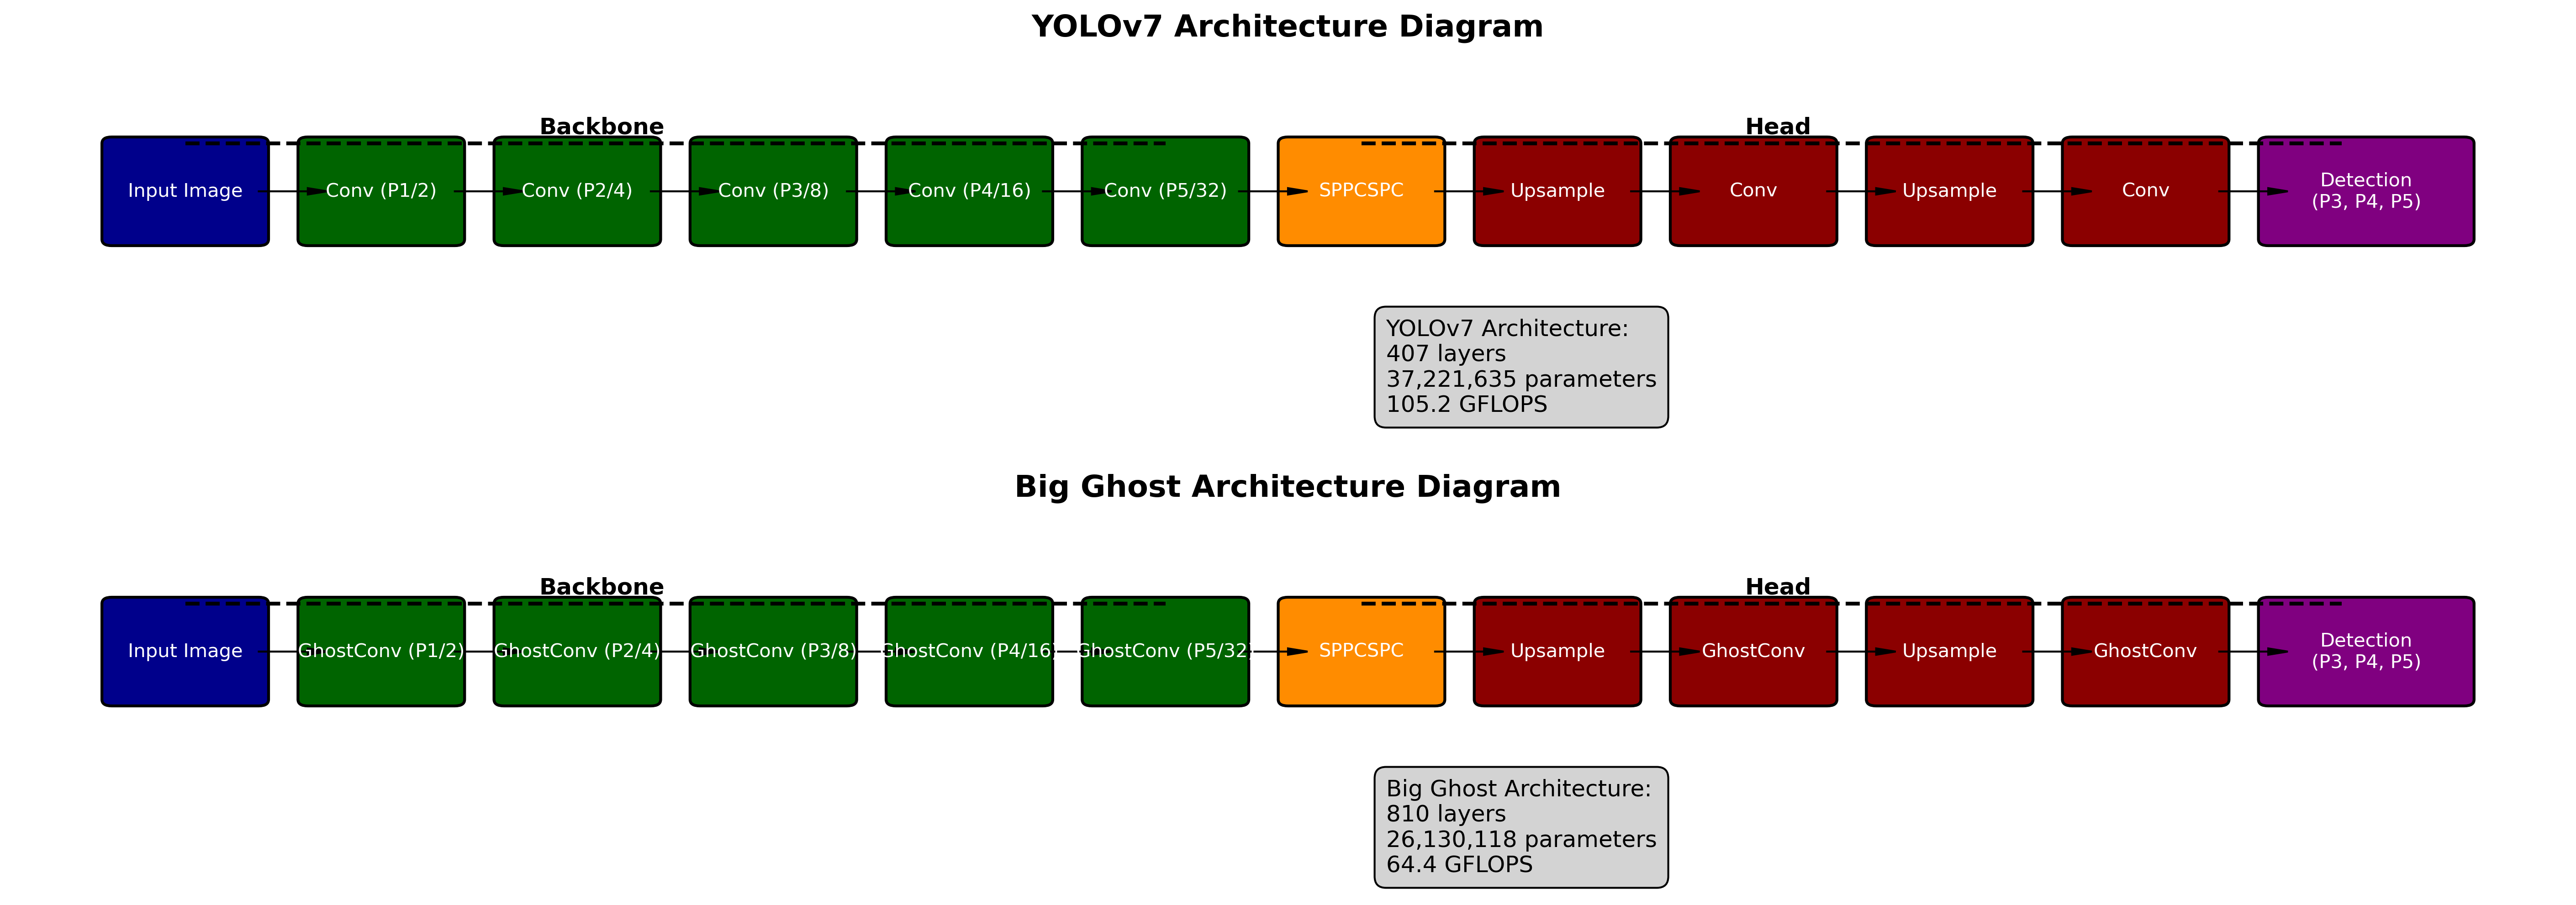
\includegraphics[width=1\linewidth]{combined_architecture.png}
    \caption{Architectural Comparison of YOLOv7 and Big Ghost: This figure shows the key differences in layers, parameters, and computational complexity between the YOLOv7 model and its Big Ghost variant.  }
    \Description{A comparison between the YOLOv7 architecture and the Big Ghost architecture, highlighting differences in layers, parameters, and computational complexity. The Big Ghost model has fewer parameters, and lower computational demands compared to YOLOv7.}
    \label{fig:yolov7_vs_big_ghost}
\end{figure*}

\begin{figure*}
    \centering
    \includegraphics[width=1\linewidth]{Screenshot 2024-08-14 at 4.14.20 PM.png}
    \caption{A graph showing the overall mAP@0.5 for each run.}
    \Description{A graph showing the overall mAP@0.5 for each run.}
    \label{fig:map05}
\end{figure*}
\begin{figure*}
    \centering
    \includegraphics[width=1\linewidth]{Screenshot 2024-08-14 at 4.14.46 PM.png}
    \caption{A graph showing the overall mAP@05:0.95 for each run}
    \Description{A graph showing the overall mAP@05:0.95 for each run}
    \label{fig:map05-95}
\end{figure*}

\begin{figure*}
    \centering
    \includegraphics[width=1\linewidth]{Screenshot 2024-08-14 at 4.15.12 PM.png}
    \caption{A graph showing the overall precision of each run}
    \Description{A graph showing the overall precision for each run}
    \label{fig:precision}
\end{figure*}

\begin{figure*}
    \centering
    \includegraphics[width=1\linewidth]{Screenshot 2024-08-14 at 4.15.31 PM.png}
    \caption{A graph showing the overall recall of each run}
    \Description{A graph showing the overall recall for each run}
    \label{fig:recall}
\end{figure*}

\bibliographystyle{ieeetr}
\bibliography{bibliography}

\end{document}